\documentclass[../statistical_learning_notes.tex]{subfiles}
\begin{document}
%%%%%%%%%%%%%%%%%%%%%%%%%%%%%%%%%%%%%%%%%%%%%%%%%%%%%%%%%%%%%%%%%%%%%%%%%%%
\section{Bias Variance Tradeoff}
In statistical learning, we learn the mapping from $X$ to $Y$, where $X$ is a matrix of size $N \times p$. $N$ denoting the number of data points we have observed, and each data point is a vector in $p$ dimensions. $Y$ is the value of the response for the observed data points and is of shape $N \times 1$. We wish to learn the mapping $f:\mathbb{R}^{p} \rightarrow \mathbb{R}$ so that we can predict the value of $Y$ for obserations where true $Y$ is not known. $(X, Y)$ is the training data avaiable to us to learn the function $f$. Additionally, there is some noise component also present in the observed $Y$
\begin{align*}
    Y = f(X) + \epsilon
\end{align*}
which is immeasureable, independent of $X$ and each other, and has $0$ mean, $E[\epsilon] = 0$. We obtain a best guess $\hat{f}$ and make predictions as
\begin{align*}
    \hat{Y} = \hat{f}(X)
\end{align*}
where $\hat{Y}$ is our best estimate of $Y$. We use least squares error to measure how good or bad our estimate $\hat{f}$ is
\begin{align*}
    E[(Y - \hat{Y})^{2}] &= E[(f(X) + \epsilon - \hat{f}(X))^{2}] = E[(f(X) - \hat{f}(X))^{2} + \epsilon^{2} + 2\epsilon f(X) - 2\epsilon \hat{f}(X)]\\
    &= E[(f(X) - \hat{f}(X))^{2}] + Var(\epsilon)\\
    Var(\epsilon) &= E[\epsilon^{2}] - E[\epsilon]^{2} = E[\epsilon^{2}]
\end{align*}
$Var(\epsilon)$ is the irreducible error since it will always be present. A good model will bring the reducible error $E[(f(X) - \hat{f}(X))^{2}]$ as close to zero as possible.\newline

Let $x_{0}$ denote a $d$ dimensional data point. The bias variance tradeoff is derived by taking expectation across $D$ datasets
\begin{align*}
    E_{D}[(y_{0} - \hat{y}_{0})^{2}] &= E_{D}[(f(x_{0}) + \epsilon - \hat{f}(x_{0}))^{2}] &= E_{D}[(f(x_{0}) + \epsilon - \hat{f}(x_{0}) + E_{D}[\hat{f}(x_{0})] - E_{D}[\hat{f}(x_{0})])^{2}]\\
    &= E_{D}[(\epsilon + (f(x_{0}) - E_{D}[\hat{f}(x_{0})]) + (\hat{f}(x_{0}) - E_{D}[\hat{f}(x_{0})]))^{2}]\\
    &= E_{D}[\epsilon^{2}] + E_{D}[(f(x_{0}) - E_{D}[\hat{f}(x_{0})])^{2}] + E_{D}[(\hat{f}(x_{0}) - E_{D}[\hat{f}(x_{0})])] + 2E_{D}[\epsilon(f(x_{0}) - E_{D}[\hat{f}(x_{0})])] + 2E_{D}[\epsilon (\hat{f}(x_{0}) - E_{D}[\hat{f}(x_{0})])] + 2E_{D}[(f(x_{0}) - E_{D}[\hat{f}(x_{0})]) + (\hat{f}(x_{0}) - E_{D}[\hat{f}(x_{0})])]\\
    &= Var(\epsilon) + (f(x_{0}) - E_{D}[\hat{f}(x_{0})])^{2} + Var(\hat{f}(x_{0})) + 0 + 0 - 2E_{D}[(f(x_{0}) - E_{D}[\hat{f}(x_{0})](E_{D}[\hat{f}(x_{0}] - E_{D}[\hat{f}(x_{0})])\\
    \Aboxed{E_{D}[(y_{0} - \hat{y}_{0})^{2}] &= Var(\epsilon) + Bias(\hat{f}(x_{0}))^{2} + Var(\hat{f}(x_{0}))}
\end{align*}
where we have used the following facts
\begin{itemize}
    \item $\epsilon$ is independent of both $f$ and $\hat{f}$\\making $E_{D}[\epsilon \times f \;or\; \hat{f}] = E_{D}[\epsilon] * constant = 0$
    \item $E[f(x_{0})] = f(x_{0})$ since $f$ is the true function and fixed/constant
    \item $E_{D}[\hat{f}(x_{0})] = constant$ and represents $\hat{f}$ averaged across all the datasets
\end{itemize}

The last equation consists of all positive terms and is called the bias variance tradeoff. $Var(\epsilon)$ is the irreducible error. Variance of $\hat{f}$ is calculated across all the datasets. The bias term represents how off our estimate is from the true value. As model flexibility increases, we get a reduction in the bias, but the variance increases, and vice versa.

\begin{figure}[h]
    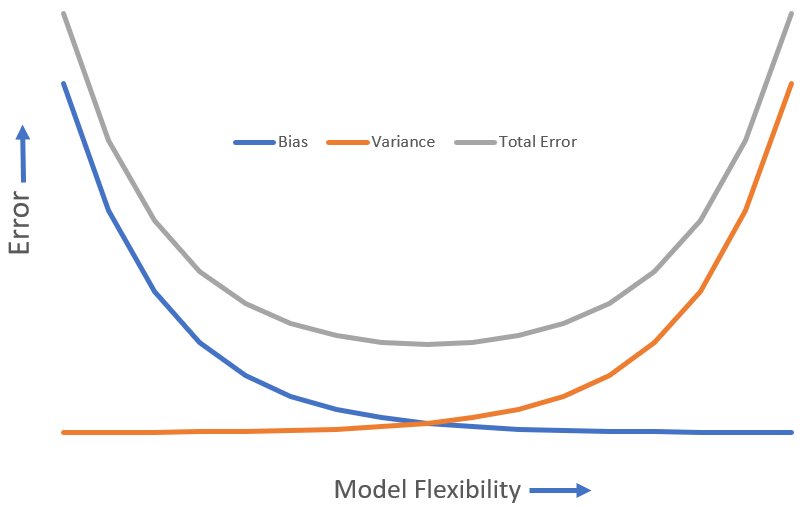
\includegraphics[scale=0.5]{bias_variance}
    \centering
    \caption {Comparison of Classifiers}
    \label{fig:bias_variance} %\ref{fig:bias_variance}
\end{figure}
\end{document}